%! suppress = LineBreak
%! suppress = MissingLabel

Как мы убедились ранее (\ref{subsec:interpreters-everywhere}), программирование состоит из написания новых и новых интерпретаторов поверх друг друга.
Интерпретаторы задают семантику новых языков (\ref{subsec:semantics}).
В классическом виде язык задаётся как множество деревьев, а интерпретатор отправляет деревья в объект мета-языка.
Если язык встроенный, то такой подход называют deep embedding (см.~\ref{subsec:edsl}).
\[
    \sembr{\bullet} : L \to D
\]

Можно заметить, что в конечном итоге мы используем только элемент домена, в который интерпретатор отображает программу.
Сама программа же представляет собой лишь удобную синтаксическую запись элемента домена и является промежуточным шагом, а не самоцелью.
В то же время доменом в случае встроенных языков, заданных интерпретаторами, являются объекты мета-языка.
Можем ли мы миновать стадию интерпретации собственного синтаксиса и сразу строить объект домена в синтаксисе мета-языка?
Да, такое встраивание называется shallow embedding, о нём эта глава.

\subsection{Формальный путь в зазеркалье} \label{subsec:to-wonderland}

Вспомним, что любую рекурсивную структуру данных можно представить как неподвижную точку функтора, задающего форму (\ref{subsubsec:functor-fixpoint}).
При этом существует универсальная свёртка, катаморфизм, которая работает для произвольного функтора формы (\ref{subsubsec:recursion-schemas}):
\begin{minted}{haskell}
    cata :: Functor f => (f a -> a) -> Fix f -> a
\end{minted}

Оказывается, что с помощью катаморфизма можно получить изоморфизм между структурами данных и их свёртками:
\mintinline{haskell}|Fix f ?$\simeq$? forall a . (f a -> a) -> a|.
\begin{minted}{haskell}
    to :: Functor f => Fix f -> (forall a . (f a -> a) -> a)
    to = flip cata

    from :: (forall a . (f a -> a) -> a) -> Fix f
    from g = g In
\end{minted}

Например, следующие два списка эквивалентны (все конструкторы \mintinline{haskell}{In} заменяем на данную алгебру):
\begin{minted}{haskell}
    data List elem rec = Nil | Cons elem rec

    xs1 :: Fix (List Int)
    xs1 = In (Cons 1 (In (Cons 2 (In (Cons 3 (In Nil))))))

    xs2 :: (List Int a -> a) -> a
    xs2 = \alg -> alg (Cons 1 (alg (Cons 2 (alg (Cons 3 (alg Nil))))))
\end{minted}

Таким образом, вместо того, чтобы конструировать дерево языка, а затем его интерпретировать (сворачивать), мы можем сразу сконструировать терм типа \mintinline{haskell}{?$\forall$?a . (f a -> a) -> a}.
Предоставив ему тип домена \texttt{a} и алгебру \texttt{f a -> a} мы немедленно получим элемент домена.

\begin{minted}{haskell}
    ghci> xs2 @Int \case Nil -> 0; Cons x acc -> x + acc
    6
\end{minted}

Однако, мы избавились ещё не от всех деревьев в программе --- остался функтор, задающий форму.
Это нерекурсивный тип, который можно представить в канонической форме (см.~\ref{subsubsec:type-algebra}):
\[
    f\ap a \iso \sum_{i}\prod_{j} (t_{ij}\ap a)
\]
Тогда алгебра может быть записана следующим образом:
\[
    f\ap a\to a\iso a^{\sum_{i}\prod_{j} (t_{ij}\ap a)} \iso \prod_{i}a^{\prod_{j} (t_{ij}\ap a)}
\]
Остались произведения, от которых можно избавиться с помощью каррирования, и получить \vocab{финальное кодирование} структуры данных\footnote{Финальным такое кодирование называется по историческим причинам. Казалось, что оно двойственно инициальному и является терминальным (финальным) объектом категории интерпретаций. Однако это не так, с категорной точки зрения, это тоже инициальный объект.}.
Например, для списка имеем:
\begin{align*}
    \text{\mintinline{haskell}{(List elem a -> a) -> a}}
    \iso a^{\displaystyle a^{\displaystyle 1 + elem\times a}}
    \iso a^{\displaystyle a\times a^{\displaystyle elem\times a}}
    \iso \left( a^{\displaystyle a} \right)^{\displaystyle \left(\left( a^{\displaystyle a}\right)^{\displaystyle elem}\right)} \\
    \iso \text{\mintinline{haskell}{a -> (elem -> a -> a) -> a}}
\end{align*}

Мы получили не что иное, как список Чёрча\footnote{\url{https://en.wikipedia.org/wiki/Church_encoding}}\footnote{\url{https://okmij.org/ftp/tagless-final/course/Boehm-Berarducci.html}}.
Структуру данных, без единого конструктора!\footnote{На самом деле в этом нет ничего удивительного, если вспомнить, что функции первого класса представляются как замыкания, содержащие данные. Мы получили тот же односвязный список, только на замыканиях.}
Перепишем знакомый нам список ещё раз:
\begin{minted}{haskell}
    xs3 :: a -> (Int -> a -> a) -> a
    xs3 = \ini f -> f 1 (f 2 (f 3 ini))
\end{minted}

Попробуем интуитивно понять, что это всё значит.
Заметим, что список Чёрча принимает функции, соответствующие веткам паттерн-матчинга или аргументам сворачивающей функции.
Вместо конструкторов же сразу вызываются соответствующие функции.
То есть, вместо того, чтобы создать структуру данных и доставить её к месту деконструирования, мы \point{доставляем место деконструирования к месту конструирования} и оказывается, что ничего конструировать по итогу и не надо.

Если зафиксировать интерпретацию, то функции-аргументы можно реализовать статически и просто ссылаться на них в терме.
Таким образом, про объявление функций можно думать как про расширение некоторого встроенного предметного языка.
Общие рассуждения про shallow embeddings, свёртки и библиотеки можно почитать в~\cite{gibbons2013functional, gibbons2014folding}.
Сравните:
\begin{figure}[h]
    \centering
    \begin{tabular}{|p{0.45\linewidth}|p{0.45\linewidth}|}
        \hline
        Deep                                                                                                                                 & Shallow                                                                              \\
        \hline
        Синтаксис языка задаётся набором допустимых нод дерева                                                                               & Декларация функции задаёт новую ноду дерева: вызов этой функции                      \\
        \hline
        Интерпретатор при виде каждой ноды выполняет соответствующий код на мета-языке (ветку паттерн-матчинга) после вычисления поддеревьев & Интерпретатор при виде вызова выполняет код тела функции после вычисления аргументов \\
        \hline
    \end{tabular}
\end{figure}

\subsection{Tagless final}

Вернёмся к некаррированной версии типа финальных термов, теперь это тип, принимающий кортеж функций.
А кортеж функций можно заменить на класс типов.
Тогда декларация класса будет задавать синтаксис встроенного языка, а инстансы для доменов~--- реализацию.
Этот подход называется \vocab{tagless final encoding}\footnote{\url{https://okmij.org/ftp/tagless-final/}} и фактически это кодирование данных по Чёрчу с классами типов и набором трюков~\cite{carette2007finally, kiselyov2012typed}.

Снова рассмотрим язык со сложением:
\begin{minted}{haskell}
    data Expr = Const Int | Plus Expr Expr

    eval :: Expr -> Int
    eval = \case Const x -> x; Plus l r -> eval l + eval r
\end{minted}
Или через катаморфизм:
\begin{minted}{haskell}
    data FExpr rec = Const Int | Plus rec rec

    eval :: Fix FExpr -> Int
    eval = cata \case Const x -> x; Plus l r -> l + r
\end{minted}
Соответствующее tagless final кодирование будет выглядеть следующим образом:
\begin{minted}{haskell}
    class Expr domain where
      cnst :: Int -> domain
      plus :: domain -> domain -> domain

    instance Expr Int where
      cnst x = x
      plus l r = l + r
\end{minted}

Теперь мы можем сконструировать обычный терм Haskell, задать домен, и машинерия классов типов подставит нужную алгебру самостоятельно:
\begin{minted}{haskell}
    example :: forall domain . Expr domain => domain
    example = cnst 1 `plus` cnst 41

    ghci> example :: Int
    42
\end{minted}

Чтобы добавить ещё интерпретацию, реализуем инстанс для другого домена:
\begin{minted}{haskell}
    instance Expr String where
      cnst x = show x
      plus l r = l <> " + " <> r

    ghci> example :: String
    "1 + 41"
\end{minted}

\subsubsection{Expression problem: произведение алгебр}

Ранее, мы пытались решить expression problem путём композирования функторов формы с помощью открытого копроизведения, а также композирования алгебр (см.~\ref{subsec:functor-coprod}).
Перейдя к финальной версии того же самого, композирование становится намного эффективнее и удобнее.
Вместо копроизведения функторов теперь имеем произведение алгебр, представляемое контекстом классов типов.

Чтобы определить ещё одну конструкцию, просто задаём новый класс с желаемыми интерпретациями:
\begin{minted}{haskell}
    class Input domain where
      input :: domain

    instance Input (Int -> Int) where
      input = \env -> env
\end{minted}

Теперь нужно снова не забыть реализовать предыдущие операции \mintinline{haskell}{Expr} для нового домена \mintinline{haskell}{Int -> Int} и можно не лету композировать языки:
\begin{minted}{haskell}
    example :: forall domain . (Expr domain, Input domain) => target
    example = cnst 1 `plus` input

    ghci> (example :: Int -> Int) 41
    42
\end{minted}

\subsubsection{Typed tagless final interpreter}

Рассмотрим наш пример tagless initial encoding~\ref{subsubsec:typed-initial}:
\begin{minted}{haskell}
    data Expr ty where
      Const :: Int -> Expr Int
      IsZero :: Expr Int -> Expr Bool
      If :: forall ty . Expr Bool -> Expr ty -> Expr ty -> Expr ty

    eval :: Expr ty -> ty
    eval = \case
      Const x  -> x
      IsZero t -> eval == 0
      If c t e -> if eval c then eval t else eval e
\end{minted}
Чтобы получить final encoding, параметризуем домен результирующим типом выражения:
\begin{minted}{haskell}
    class Expr (domain :: Type -> Type) where
      cnst :: Int -> domain Int
      isZero :: domain Int -> domain Bool
      if' :: forall ty . domain Bool -> domain ty -> domain ty -> domain ty

    class Expr Identity where
      cnst x = Identity x
      isZero (Identity x) = Identity (x == 0)
      if' (Identity c) t e = if c then t else e
\end{minted}

\begin{task}
    Какой домен подойдёт для печати выражения?
\end{task}

Можно сделать константы полиморфными, но тогда разумно дать возможность реализациям наложить ограничения на их полиморфизм.
Добьёмся этого с помощью ассоциированного семейства констреинтов:
\begin{minted}{haskell}
    class Expr domain where
      type C domain ty :: Constraint
      val :: C domain ty => ty -> domain ty
      -- ...

    instance Expr Identity where
      type C Identity ty = ()
      val x = Identity x
      -- ...

    instance Expr (Const String) Where
      type C (Const String) ty = Show ty
      val x = Const $ show x
      -- ...

    example :: forall domain . (C domain ty, Expr domain) => domain ty
    example = val 42

    ghci> example :: Const String Int
\end{minted}

\subsubsection{Встречаем старых друзей}

Рассмотрим следующий язык в initial encoding с higher order abstract syntax (см.~\ref{subsubsec:h-syntax}:
\begin{minted}{haskell}
    data Expr s ty where
      Val :: ty -> Expr s ty
      App :: Expr s (arg -> res) -> Expr s arg -> Expr s res
      LetIn :: Expr s ty -> (ty -> Expr s ty') -> Expr s ty'
      Get :: Expr s s
      Put :: s -> Expr s ()

    modify :: (s -> s) -> Expr s s
    modify f =
      Get `LetIn` \x ->
      Val (const x) `App` Put (f x)
\end{minted}

Перепишем в tagless final, выбирая подходящие имена для кусков синтаксиса:
\begin{minted}{haskell}
    class Applicative domain where
      pure :: ty -> domain ty
      (<*>) :: domain (arg -> res) -> domain arg -> domain res

    class Monad domain where
      (>>=) :: domain ty -> (ty -> domain ty') -> domain ty'

    class MonadState s domain | domain -> s where
      get :: domain s
      put :: s -> domain ()
\end{minted}

Таким образом, аппликативные функторы --- meta-circular язык с аппликацией, а монадический bind --- это фактически let-in в higher-order синтаксисе.

Реализуем знакомую интерпретацию для подходящего домена:
\begin{minted}{haskell}
    newtype State s a = State { runState :: s -> (s, a) }

    instance Applicative (State s) where
      pure x = State \s -> (s, x)
      State fs <*> State xs = State \s1 ->
        let (s2, f) = fs s1 in let (s3, x) = xs s2 in (s3, f x)

    instance Monad (State s) where
      State comp >>= k = State \s ->
        let (s', x) = comp s in runState (k x) s'

    instance MonadState s (State s) where
      get = State \s -> (s, s)
      put s' = State \s -> (s', ())
\end{minted}

\subsubsection{Восстановление композиционности семантики} \label{subsubsec:recover-compositionality}

\vocab{Семантика} называется \vocab{композиционной}, если значение сложного выражения определяется его структурой и семантикой его подструктур. % todo ref back

Всякие преобразования кода не композиционные.
Для примера рассмотрим протаскивание унарных отрицаний:
\begin{minted}{haskell}
    data Expr1 = Lit Int | Add Expr1 Expr1 | Neg Expr1 deriving Show

    transform1 :: Expr1 -> Expr1
    transform1 = \case
      Lit x -> Lit x
      Neg (Lit x) -> Lit (-x)
      Add l r -> Add (transform1 l) (transform1 r)
      Neg (Neg e) -> transform1 e
      Neg (Add l r) -> Add (transform1 (Neg l)) (transform1 (Neg r))
\end{minted}

Чтобы восстановить композиционность семантики, нужно экплицировать контекстные зависимости с помощью функционального домена:
\begin{minted}{haskell}
    class Expr2 d where
      lit :: Int -> d
      add :: d -> d -> d
      neg :: d -> d

    data Ctx = CtxPos | CtxNeg

    instance Expr2 d => Expr2 (Ctx -> d) where
      lit x CtxNeg = lit (-x)
      lit x CtxPos = lit x
      neg e CtxNeg = e CtxPos
      neg e CtxPos = e CtxNeg
      add l r ctx = add (l ctx) (r ctx)
\end{minted}





%\subsubsection{Tagless final meta-circular evaluator}
%
%Повторим рассмотренный ранее язык в tagless final стиле.
%
%\begin{minted}{haskell}
%     data Term3 ty where
%       Val3 :: ty -> Term3 ty
%       Plus :: Term3 Int -> Term3 Int -> Term3 Int
%       App3 :: Term3 (arg -> res) -> Term3 arg -> Term3 res
%       Lam3 :: (Term3 arg -> Term3 res) -> Term3 (arg -> res)
%
%     example3 :: Term3 Int
%     example3 = (Lam3 \x -> x `Plus` Val3 41) `App3` Val3 1
%
%     eval3 :: Term3 ty -> ty
%\end{minted}
%
%\begin{minted}{haskell}
%    class Term d where
%      type C d ty :: Constraint
%      val :: C d ty => ty -> d ty
%      plus :: d Int -> d Int -> d Int
%      app :: d (arg -> res) -> d arg -> d res
%      lam :: (d arg -> d res) -> d (arg -> res)
%
%    example :: (Term d, C d Int) => d Int
%    example = (lam \x -> x `plus` val 41) `app` val 1
%
%    instance Term Identity where
%      type C Identity ty = ()
%      val = Identity
%      plus = liftA2 (+)
%      app = liftA2 ($)
%      lam = coerce
%
%    instance Term (Const String) where
%      type C (Const String) ty = Show ty
%      val = Const . show
%      plus (Const l) (Const r) = Const $ "(" ++ l ++ " + " ++ r ++ ")"
%      app (Const f) (Const arg) = Const $ "(" ++ f ++ " " ++ arg ++ ")"
%      lam f = Const $ "(" ++ "\\x -> " ++ getConst (f (Const "x")) ++ ")"
%\end{minted}
%
%TODO % todo
%



%
%TODO % todo
%
%% todo bananas in space и что там было про функции и зачем
%
%\subsection{Зазеркалье в реальности}
%
%\subsubsection{Expression problem}
%
%\url{https://homepages.inf.ed.ac.uk/wadler/papers/expression/expression.txt}
%
%% todo wadler the expression problem
%
%% todo Extensibility for the Masses: Practical Extensibility with Object Algebras
%
%TODO % todo
%
%\subsubsection{Deforestation \& fusion}
%
%\vocab{Дефорестация} --- процесс избавления программы от (промежуточных) деревьев~\cite{wadler1988deforestation} (рис.~\ref{fig:deforestation-examples}).
%Дефорестация является частным случаем суперкомпиляции~\cite{supercomp}.
%
%\begin{figure}
%    \centering
%    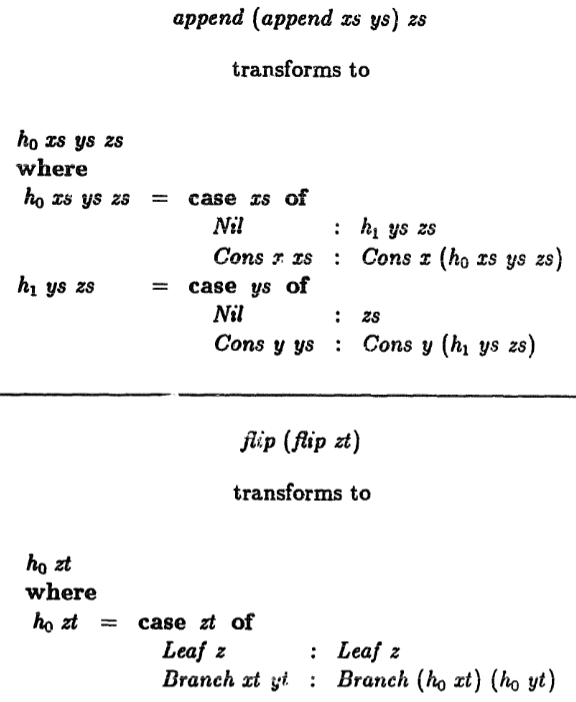
\includegraphics[width=0.55\textwidth]{figs/deforestation-examples}
%    \caption{Примеры работы дефорестирующего алгоритма~\cite{wadler1988deforestation}.}
%    \label{fig:deforestation-examples}
%\end{figure}
%
%Однако, алгоритм дефорестации имеет проблемы: он либо имеет шанс не завершиться на рекурсивных определениях, либо ограничен программами очень специального вида.
%Поэтому для Haskell был предложен другой способ, работающий только на списках, дефорестирующий с помощью алгебраических свойств списочных трансформаций\footnote{\url{https://markkarpov.com/tutorial/ghc-optimization-and-fusion.html}}~\cite{gill1993short}.
%
%Вместо использования множества алгебраических правил, определяем универсальный способ конструирования и деконструирования списка.
%Деконструируем с помощью \mintinline{haskell}|foldr|:
%\begin{minted}{haskell}
%    foldr f ini . map g ?$\equiv$? foldr (f . g) ini
%\end{minted}
%
%Конструируем с помощью \mintinline{haskell}|build|.
%Можно заметить, что на вход передаётся список Чёрча, отсюда не удивителен закон:
%\begin{minted}{haskell}
%    build :: (forall b . (a -> b -> b) -> b -> b) -> [a]
%    build g = g (:) []
%
%    foldr f ini (build g) ?$\equiv$? g f ini
%\end{minted}
%
%% todo \cite{meijer1991functional}
%
%TODO % todo пример
%
%\subsubsection{Streams \& reactive programming}
%
%Если пойти в обратную сторону относительно анаморфизма, то получим структуру данных, заданную через развёртку.
%Такая структура даже в энергичном языке может быть потенциально бесконечной.
%\begin{minted}{haskell}
%    anaInv :: Fix f -> ?$\exists$?s . (s -> f s, s)
%\end{minted}
%
%TODO\cite{coutts2007stream, kiselyov2022highest} % todo stream fusion from lists to streams to nothing at all
%
%% todo Reading circle about fusion
%
%% todo haskell inlining
%% todo Oleg about fusion and streams
%
%% todo call-pattern specialization for Haskell programs
%
%% todo FRP
%% todo reactive programming https://youtu.be/sTSQlYX5DU0?si=Ybxux16h5Vt1LnC4
%
%% todo internal iteration
%
%TODO % todo
%
%\subsubsection{Data vs codata}
%
%\url{https://reasonablypolymorphic.com/blog/review-codata/index.html}
%
%% todo codata, copattern-matching
%% todo are custom patterns in haskell connected to this?
%
%% todo когда использовать дату, а когда - кодату (интерпретируем входые данные)
%
%TODO~\cite{downen2019codata} % todo
%
%\subsubsection{Threaded code}
%
%TODO % todo https://en.wikipedia.org/wiki/Threaded_code
%
%% todo pull and push
%
%% todo \vocab{полярности}\footnote{\url{https://existentialtype.wordpress.com/2012/08/25/polarity-in-type-theory/}}\footnote{\url{https://ncatlab.org/nlab/show/polarity+in+type+theory}}

%Можно заметить, что термы в зазеркалье можно представлять как объекты с единственным методом \texttt{visit}, а инстанс соответствующего класса типов --- visitor.
%
%% todo visitor pattern

% todo зафиксировать где-то достижение, что код пишется на нормальном хаскеле
